\documentclass[]{beamer}
% \geometry{papersize={16cm,9.60cm}}
\usepackage{etex}
\usepackage{amsmath}
\usepackage{tikz}
\usepackage{multimedia}
\usetheme{Boadilla}
\usepackage{graphicx}
\usepackage{url}

%\usepackage{inputenc}

% \mode<presentation>
% {
%   \usetheme{default}
%   \setbeamercovered{transparent}
% }


% {\vskip5pt}

%% customize layout, bullet points navigation toolbar
\setbeamertemplate{navigation symbols}{}%remove navigation symbols
\setbeamertemplate{enumerate items}[default]
\setbeamertemplate{navigation symbols}{}
\setbeamertemplate{itemize items}[circle]
\setbeamercolor{enumerate item}{fg=black}

\setbeamertemplate{footline}{}
\setbeamersize{text margin left = 2.0em}
\setbeamersize{text margin right = 2.0em}


\usepackage{times}
\usepackage[T1]{fontenc}

% Or whatever. Note that the encoding and the font should match. If T1
% does not look nice, try deleting the line with the fontenc.

\setbeamertemplate{navigation symbols}{}

\title{ Cognitive (Neuro) Psychology }
\subtitle{XI. Judgement and Decision Making}
\author{ Marianne Maertens }
\institute[TU Berlin]{Technische Universit\"at Berlin}
\date{September 2016}

\begin{document}
\setbeamertemplate{enumerate items}[default]
\setbeamertemplate{headline}

\frame{\titlepage}

\AtBeginSection[]
{
  \begin{frame}<beamer>
    \frametitle{Layout}
    \tableofcontents[currentsection]
  \end{frame}
}

\begin{frame}
 \frametitle{Judgement and decision making}
\begin{overlayarea}{130mm}{70mm}
... are one of many forms of thinking
\
\begin{columns}[T]
 \begin{column}{50mm}
\begin{center}
\begin{itemize}
 \item<2-> plan and solve our daily problems
 \item<2-> solve a newspaper puzzle
 \item<2-> troubleshooting when your bike breaks down
 \item<2-> write a bachelor thesis
 \item<3-> decide on breakfast
 \item<4-> determines your experiences $\Rightarrow$ shapes your \textbf{personality}
\end{itemize}
\end{center}
 \end{column}
 \begin{column}{70mm}
\vspace{5mm}
\includegraphics<2>[width=50mm]{figs/l11/sudoku.png}
\includegraphics<3>[width=50mm]{figs/l11/wafflehouse.jpg}
\includegraphics<4>[width=50mm]{figs/l11/fit_person.jpg}
 \end{column}
\end{columns}
\end{overlayarea}
 \end{frame}


\begin{frame}
\frametitle{Judgement and decision making}
 \begin{overlayarea}{110mm}{60mm}
\textbf{Decision making}
\begin{itemize}
 \item selecting one out of a number of possible options with the decision having personal consequences, emphasis on importance of the decision
 \end{itemize}

\only<2->{
\vspace{3mm}
\textbf{Judgement}
 \begin{itemize}
 \item a component of decision making that involves calculating the likelihood of various possible events using incomplete information, emphasis on accuracy
 \begin{itemize}
 \item<3-> difficulty of an exam
 \item<3-> outcome of an election 
 \item[]
 \item<4-> ``I think that...'', ``chances are ...'', ``it is unlikely that ...''
 \item[]
\end{itemize}

\item<5->[$\Rightarrow$] \textcolor{blue}{How do people assess the probability of an uncertain event?}
\end{itemize}
}
\end{overlayarea}
\end{frame}



\begin{frame}
\frametitle{Judgement and decision making}
 \begin{overlayarea}{110mm}{80mm}

The subjective assessment of probabilities resembles the \textit{subjective assessment} of physical quantities such as distance or size. 

 \centering
\includegraphics<1->[width=50mm]{figs/l11/aerial_perspective.jpg}

 \begin{itemize}
 \item<2-> \textit{apparent distance} of an object partly determined by its \textit{perceived clarity}: the more sharp the closer it appears
 \item<3-> sharpness \textbf{cue} to distance 
 \item<4-> might lead to systematic \textbf{errors} because there might be other reasons for blurriness than distance
\end{itemize}

\end{overlayarea}
\end{frame}


\begin{frame}
 \frametitle{Outline}
\begin{itemize}[<+->]
  \setlength{\itemsep}{5pt}
 \item Judgement research
 \item Probabilites and judgement
 \item Heuristics and biases
 \item Judgement theories
 \item Decision making under risk
\end{itemize}
\end{frame}

\begin{frame}
 \frametitle{Taxi-cab problem}
\begin{overlayarea}{110mm}{80mm}
 \begin{columns}[T]
 \begin{column}{60mm}
 \begin{center}
\includegraphics<1>[width=60mm]{figs/l11/taxi_cab_1.png}
\includegraphics<2>[width=60mm]{figs/l11/taxi_cab_2.png}
\includegraphics<3->[width=60mm]{figs/l11/taxi_cab_3.png}
 \end{center}
 \end{column}

 \begin{column}{50mm}
\begin{center}
\begin{itemize}
 \item<4->[!] tested under similar visibility conditions, the witness was \textbf{wrong 20\%} of the time
 \item<5->[?] Given all the information what is the \textbf{probability} that the cab involved in the accident was \textcolor{blue}{blue}?
\end{itemize}
\end{center}
 \end{column}
\end{columns}
\begin{itemize}
 \item[]
 \item<6->[$\Rightarrow$] majority of participants: 
 \item<6->[] \textit{80\% likelihood} that the cab was \textcolor{blue}{blue}!
\end{itemize}

\end{overlayarea}
\end{frame}


\begin{frame}
 \frametitle{Taxi-cab problem - probability theory}
\begin{overlayarea}{110mm}{80mm}
 \begin{columns}[T]
 \begin{column}{50mm}
 \centering
\includegraphics<1>[width=50mm]{figs/l11/taxi_cab_2.png}
\includegraphics<2->[width=45mm]{figs/l11/taxi_cab_3a.png}\\
 \end{column}

 \begin{column}{70mm}
 \centering
\includegraphics<1>[width=70mm]{figs/l11/taxi_cab_4.png}
\includegraphics<2>[width=70mm]{figs/l11/taxi_cab_5.png}
\includegraphics<3,6->[width=70mm]{figs/l11/taxi_cab_6.png}
\includegraphics<4-5>[width=70mm]{figs/l11/taxi_cab_7.png}
 \end{column}
\end{columns}

\only<4->{
\begin{itemize}
 \item[?] $P(\textcolor{blue}{blue}|``blue")$ 
\end{itemize}
}
\only<5->{$\Rightarrow$ \textbf{Bayes' rule:}\\}
\only<5->{
\vspace{2mm}
$P(\textcolor{blue}{blue}|``blue")=\frac{P(``blue"|\textcolor{blue}{blue}) * P(\textcolor{blue}{blue})}{P(``blue" |\textcolor{blue}{blue}) * P(\textcolor{blue}{blue}) + P(``blue"|\textcolor{green}{green})  * P(\textcolor{green}{green})}$
}

\only<6->{
\vspace{2mm}
$P(\textcolor{blue}{blue}|``blue")=\frac{.8 * .15}{.8 * .15 + .2 * .85}=\frac{.12}{.12+.17}=\frac{.12}{.29}=.41$}

\only<7->{
\vspace{5mm}
vs. 80\% likelihood judged by subjects = \textbf{base rate fallacy}\\ \vspace{2mm}
people's tendency to ignore the relative frequency with which an event occurs within a population

}
\end{overlayarea}
\end{frame}

\begin{frame}{Terminology}
 \begin{overlayarea}{110mm}{80mm}
\centering
  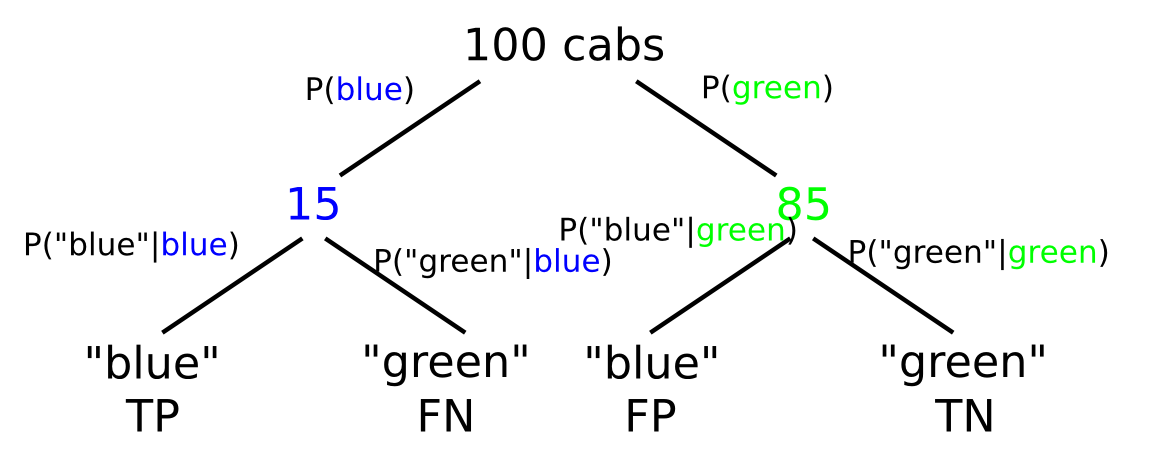
\includegraphics[width=70mm]{figs/l11/taxi_cab_7.png}
\begin{columns}[T]
\begin{column}{70mm}
\begin{itemize}
 \item TP - true positive, hit
 \item FN - false negative, miss
 \item FP - false positive, false alarm
 \item TN - true negative, correct rejection
 \item[]
 \item Sensitivity = $\frac{TP}{TP+FN}$
 \item Specificity = $\frac{TN}{TN+FP}$ 
\end{itemize}
\end{column}
\begin{column}{40mm}
  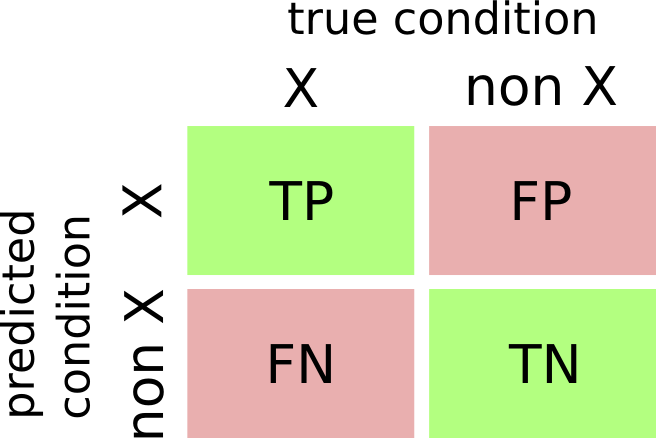
\includegraphics[width=40mm]{figs/l11/contingency.png} 
\end{column}
 \end{columns}

 \end{overlayarea}
\end{frame}


\begin{frame}
 \frametitle{Heuristics}
\begin{overlayarea}{110mm}{80mm}
Tversky and Kahneman, 1974
 \begin{itemize}
 \item strategies that ignore part of the information, with the goal of making decisions more quickly, simple, and/or accurately than more complex methods 
 \item reduce effort associated with a task
 \item rules of thumb = cues
 \item lead to errors
 \end{itemize}
\end{overlayarea}
\end{frame}


\begin{frame}
 \frametitle{Representativeness heuristic}
\begin{overlayarea}{110mm}{80mm}
 What is the probability that object A belongs to class B?\\
What is the probability that event A originates from process B?\\
\begin{itemize}
 \item<2->[$\Rightarrow$] Representativeness heuristic:
 \item<2->[] probabilities are evaluated by the degree to which A resembles B
\end{itemize}
\only<3->{
\begin{block}{Steve}
\begin{small}
is shy and withdrawn, invariably helpful, but with little interest in people, or in the world of reality. A meek and tidy soul, he has a need for order and structure, and a passion for detail. Steve is most likely a ...\end{small}
\begin{enumerate}
\begin{small}
 \item Farmer
 \item Salesman
 \item Airline pilot
 \item Librarian
 \item Physician
\end{small}
\end{enumerate}
\end{block}
}
\end{overlayarea}
\end{frame}


\begin{frame}
 \frametitle{Representativeness heuristic - Errors}
\begin{overlayarea}{110mm}{80mm}
\textit{Insensitivity to prior probability of outcomes\\ \vspace{3mm}}
\textbf{Experiment:}
\begin{itemize}
 \item brief personality descriptions
 \item allegedly sampled at random from a group of 100 professionals: lawyers and engineers
 \item two conditions: lawyers:engineers = 70:30 OR 30:70
 \item<2->[$\Rightarrow$] subjects produced identical probability judgements (ignoring base rates!)
 \item<3->[a] absence of personality sketch $\Rightarrow$ probabilities judged according to base rates
 \item<4->[b] uninformative personality description:
 \item<4->[]\begin{tiny} Dick is 30y old. Married with no children. Man of high ability and high motivation, he promises to be quite successful in his field. Is well liked by his colleagues.\end{tiny}
 \item<5->[$\Rightarrow$] P(Dick|engineer)=.5
\end{itemize}
\end{overlayarea}
\end{frame}


\begin{frame}
 \frametitle{Representativeness heuristic - Errors}
\begin{overlayarea}{110mm}{70mm}
\textit{Gambler's fallacy}

\begin{itemize}
 \item imagine a coin has been tossed 6 times in succession
 \item in the first run we observe the sequence: H-T-H-T-T-H, in the second run we observe the sequence: H-H-H-H-H-H
 \item[$\Rightarrow$] Which one is more likely?
 \item<2-> people judge H-T-H-T-T-H to be more likely, as this sequence better represents the intuitive description of a random sequence
 \item<3-> a long sequence of heads does not mean that tail is now due = \textbf{Gambler's fallacy}

\end{itemize}
\end{overlayarea}
\end{frame}


\begin{frame}
 \frametitle{Representativeness heuristic - Errors}
\begin{overlayarea}{110mm}{80mm}
\textit{Illusion of validity}

\begin{itemize}
 \item predict grade point average for students:
 \item student A: 2,2,1,2,2,3,2,2
 \item student B: 1,3,1,3,2,4,1,1
 \item<2->[$\Rightarrow$] higher confidence in consistent pattern
\end{itemize}

\only<3->{
\textit{Misconception of regression}

\begin{columns}[T]
 \begin{column}{50mm}
\centering
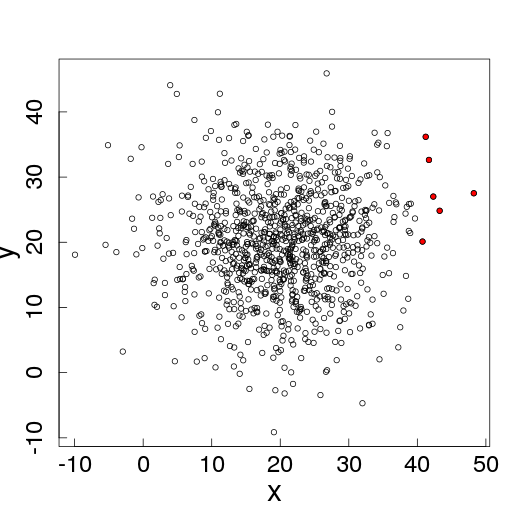
\includegraphics[width=45mm]{figs/l11/regression_to_mean.png}
 \end{column}

 \begin{column}{60mm}
\begin{itemize}
 \item regression toward the mean
 \item e.g. flight training: praise for an exceptionally good landing $\rightarrow$ poorer landing
\end{itemize}
 \end{column}
\end{columns}
}
\end{overlayarea}
\end{frame}



\begin{frame}
 \frametitle{Availability heuristic}
\begin{overlayarea}{110mm}{70mm}
Probabilities are evaluated by the ease with which instances or occurrences can be brought to mind
\begin{itemize}
 \item \textit{Availability} useful clue for assessing frequency or probability, because instances of large classes are usually recalled better and faster than instances of less frequent classes
\end{itemize}


\begin{columns}[T]
 \begin{column}{50mm}
\begin{itemize}
 \item<2->[$\rightarrow$] Which is more likely?
 \item<2->[] \underline{r} \underline{ }  \underline{ }
 \item<2->[] \underline{ } \underline{ }  \underline{r}
\end{itemize}
 \end{column}

 \begin{column}{60mm}
\begin{itemize}
 \item<3-> it is easier to search for words by their first letter
 \item<3->[$\Rightarrow$] people judge words that begin with ``r" to be more numerous although it is more frequent in the 3rd than in the 1st position 
\end{itemize}
 \end{column}
\end{columns}
\only<4->{
\begin{center}
\textit{Bias due to effectiveness of search set}
\end{center}
}
\end{overlayarea}
\end{frame}


\begin{frame}
 \frametitle{Adjustment and anchoring}
\begin{overlayarea}{120mm}{70mm}
 Probabilities are evaluated starting from and initial value and making adjustments to yield the final answer\\ \vspace{3mm}
\textit{Insufficient adjustment} 
\begin{itemize}
 \item Estimate the product (5sec): 
 \item<2,6-> 1 x 2 x 3 x 4 x 5 x 6 x 7 x 8 = \only<6->{512}
 \item<3,5> answer? 
 \item<4,6-> 8 x 7 x 6 x 5 x 4 x 3 x 2 x 1 = \only<6->{2.250}
 \item<7-> correct answer: 40.320
 \item[]
 \item<8-> people perform a few steps of computation and estimate the product by extrapolation $\rightarrow$ underestimation
\end{itemize}
\end{overlayarea}
\end{frame}

\begin{frame}{Evaluation}
 \begin{overlayarea}{120mm}{80mm}
  
\begin{itemize}
 \item Kahneman and Tversky did groundbreaking work in establishing several heuristics that underlie judgements in different contexts
 \item plentiful of evidence that humans prefer to mimize cognitive demands on them by using heuristics
 \item[]
 \item<2->[!] heuristics were vaguely defined - one-world labels and theory substitutes that fail to place any testable constraints on the cognitive decision process
 \item<3->[!] much research is detached from the realities of everyday life, emotional and motivational factors often influences our judgements in the real world
 \item<4->[!] sometimes unfair to conclude people's judgements are biased, e.g. skin cancer is judged to be a more common cause of death than cancer of mouth and throat, however, skin cancer has received more media coverage 
 \end{itemize}
\end{overlayarea}
\end{frame}



\begin{frame}
 \frametitle{Judgement theories}
\begin{overlayarea}{110mm}{80mm}
 \textbf{Support theory} (Tversky and Kohler, 1994)
\begin{itemize}
 \item event appears more or less likely depending on how it is described
 \item<2->[$\rightarrow$] distinction between \textit{event} and \textit{description} of it, e.g.
 \begin{itemize}
  \item<3-> probability of dying in my next summer holiday?
  \item<3-> probability of dying because of diving accident, fall when hiking, food poisoning, plane crash, ...?
  \item<3->[$\Rightarrow$] subjective probability judged higher for specific description
 \end{itemize}
 \item<4-> explicit description draws attention to aspects of the event that are otherwise less obvious 
 \item<4->[$\rightarrow$] increases number of instances in class 
 \item<4->[$\rightarrow$]  \textit{availability heuristic:} class size $~$ probability
 \item[]
 \item<5->[!] explicit description may reduce subjective probability if they lead individuals to focus on low-probability causes
\end{itemize}
\end{overlayarea}
\end{frame}



\begin{frame}
 \frametitle{Judgement theories}
\begin{overlayarea}{110mm}{80mm}
 \textbf{Natural frequency hypothesis} (Gigerenzer and Hoffrage, 1999)
\begin{itemize}
 \item people are rarely presented with base-rate information
 \item instead: natural sampling
 \item[$\rightarrow$] easier to work out the \textit{frequency} of different events than \textit{fractions} or percentages
 \item<2->[$\rightarrow$] performance on judgement problems should be enhanced when frequency information is used
\end{itemize}
\end{overlayarea}
\end{frame}


\begin{frame}
\textbf{Probability format:} The probability of breast cancer is 1\% for women at
age forty who participate in routine screening. If a woman has breast
cancer, the probability is 80\% that she will get a positive mammography.
If a woman does not have breast cancer, the probability is 9.6\% that she
will also get a positive mammography. A woman in this age group had a
positive mammography in a routine screening. What is the probability
that she actually has breast cancer?\\ \vspace{3mm}

\textbf{Frequency format:} 10 out of every 1,000 women at age forty who
participate in routine screening have breast cancer. 8 of every 10 women
with breast cancer will get a positive mammography. 95 out of every 990
women without breast cancer will also get a positive mammography.
Here is a new representative sample of women at age forty who got a
positive mammography in routine screening. How many of these women
do you expect to actually have breast cancer?\\
\end{frame}



\begin{frame}
 \frametitle{Judgement theories}
\begin{overlayarea}{110mm}{80mm}
 \textbf{Natural frequency hypothesis} (Gigerenzer and Hoffrage, 1999)
\begin{itemize}
 \item people are rarely presented with base-rate information
 \item instead: natural sampling
 \item[$\rightarrow$] easier to work out the \textit{frequency} of different events than \textit{fractions} or percentages
 \item[$\rightarrow$] performance on judgement problems should be enhanced when frequency information is used
 \item[]
 \item[$\Rightarrow$] Performance is considerably higher with the frequency format (Fiedler et al., 2000) 
\item[]
 \item<2->[!] potential confound - frequency version of the problem make the underlying problem structure more obvious
\end{itemize}
\end{overlayarea}
\end{frame}

\begin{frame}
\frametitle{Decision making under risk}
\begin{overlayarea}{110mm}{80mm}
Life is full of decisions
\begin{itemize}
 \item Which movie will I see tonight?
 \item Would I prefer to learn Italian or Spanish?
 \item Who will I share an apartment with next year?
\end{itemize}
\only<2->{
\vspace{2mm}
Assumption: 
\begin{itemize}
 \item people behave rationally - theories on how people \textit{should} make decision and not how they \textit{actually} make them
\end{itemize}
}

\only<3->{
\vspace{2mm}
\textbf{Utility theority} (von Neumann and Morgenstern, 1944)
\begin{itemize}
 \item[] $Expected\_Utility = P(outcome A) * Utility(outcome A)$
 \item people try to maximize utility, i.e. subjective value attached to each outcome 
\end{itemize}
}
\end{overlayarea}
\end{frame}


\begin{frame}
\frametitle{Decision making under risk}
\begin{overlayarea}{115mm}{80mm}
 Kahneman and Tversky, 1984
\begin{itemize}
 \item gamble - toss a coin: 2 ways to play the game
 \begin{itemize}
  \item if heads comes up you surely gain 800\$
  \item if heads comes up you have an 85\% chance of gaining 1000\$ and a 15\% of gaining nothing 
 \end{itemize}
 \item<2-> expected gain is greater for the latter decision
 \item<2-> $\frac{2}{3}$ of the subjects choose safe option (smaller expected gain)   
\end{itemize}

\only<3->{\textbf{Prospect theory}
\begin{columns}[T]
\begin{column}{70mm}
\begin{enumerate}
 \item individuals identify a reference point that represents their current state
 \item individuals are more sensitive to potential losses than potential gains - loss aversion
 \item<4->[$\rightarrow$] unwilling to accept bets with \textit{potential} losses
\end{enumerate}
\end{column}
 
\begin{column}{40mm}
\includegraphics<3->[width=40mm]{figs/l11/value_function.png}
\end{column}
\end{columns}
}
\end{overlayarea}
\end{frame}


\begin{frame}
\frametitle{Prospect theory - Framing effects}
\begin{overlayarea}{115mm}{80mm}
 \textbf{Asian disease problem}: \textit{Imagine the US is preparing for the outbreak of an unusual Asian disease, which is expected to kill 600 people. Two alternative programs to combat the disease have been proposed. Assume that the exact scientific estimate of the consequences of the program are as follows ... }\\ \vspace{2mm}
\only<2->{
\textbf{Gain-frame} \only<4->{$\rightarrow$ 72\% chose A }

\begin{itemize}
 \item If program A is adopted, 200 people will be saved
 \item If program B is adopted, there is a 1 in 3 probability 600 people will be saved, and a 2 in 3 probability that nobody will be saved
 \end{itemize}
}
\only<3->{
\textbf{Loss-frame} \only<5->{$\rightarrow$ 78\% chose D }
\begin{itemize}
 \item If program C is adopted, 400 people will die
 \item If program D is adopted, there is a 1 in 3 probability that nobody will die, and a 2 in 3 probability that 600 people will die
 \end{itemize}
}
\end{overlayarea}
\end{frame}


\begin{frame}
\frametitle{Prospect theory - Framing effects}
\begin{overlayarea}{115mm}{80mm}
Problems with interpretation

\begin{itemize}
 \item[!] certain option more \textit{ambiguous} than the risky option - people might have interpreted program A as \textit{at least} 200 people will be saved, and program C as \textit{at least} 400 people will die
 \item<2->[$\rightarrow$] when all programs were described in detail - framing effect disappeared (Mandel and Vartanian, 2011)
 \item[]
 \item<3->[!] relevance of \textit{social and moral factors} - \underline{version:} 
 \item<4-> \textit{definite} survival of 2/3 of the patients OR 1/3 \textit{probability} of all patients surviving and 2/3 probability of none surviving
 \item<4-> deterministic option leads - on average - to survival of twice as many patients, probabilistic option seems more fair because all patients share the same fate
 \item<5->[$\Rightarrow$] deterministic option for unknown people
 \item<5->[$\Rightarrow$] probabilistic option for close relatives
\end{itemize}
\end{overlayarea}
\end{frame}



\begin{frame}
 \frametitle{Summary}
\begin{itemize}[<+->]
\setlength{\itemsep}{2pt}
 \item close relationships between areas of decision making and judgement: deciding on a course of action and its consequences vs. estimating probabilities
 \item estimate of the probability of something changes in the light of evidence, potential  failure to take base-rate information into account in part because of \textbf{representativeness} heuristic
 \item according to \textbf{support theory}, an event's subjective probability increases as its description becomes more explicit and detailed, partly due to \textbf{availability} heuristic
 \item according to the \textbf{natural frequency hypothesis}, judgements are more accurate when based on natural frequencies rather than probabilities
 \item according to \textbf{prospect theory} people are more sensitive to potential losses than to potential gains
\end{itemize}
\end{frame}



\begin{frame}
 \frametitle{References}
\begin{small}
\begin{itemize}
 \item  Eysenck, M. W. \& Keane, M.T. (2015). \textit{Cognitive Psychology. A student's handbook}. Psychology Press: Hove, East Sussex. 
\end{itemize}
\end{small}
\end{frame}


\end{document}